\documentclass[fleqn,10pt]{wlscirep}
\usepackage[utf8]{inputenc}
\usepackage{hyperref}
\usepackage[T1]{fontenc}
\usepackage{pdfpages}
\title{Title: G13ODI}
\author{Shubham Bhandari shubhambhandari13@gmail.com}
\affil[]{This is project report for the subject 'CS1305: Business Intelligence' at JK Lakshmipat University, Jaipur}

\begin{abstract}
Abstract Content
\end{abstract}

\begin{document}
\flushbottom
\maketitle
\thispagestyle{empty}

\noindent Please note: Abbreviations should be introduced at the first mention in the main text – no abbreviations lists. Suggested structure of main text (not enforced) is provided below.

\section{Introduction}

\section{Background}
\subsection{The Game of Cricket}
'Cricket' also known as 'Gentlemen's game' is a bat and ball team sport played between two teams of eleven players each. 
The game is played on a ground at the centre of which is a 22-yard pitch with three wooden stumps at both the ends known as wickets.
The wickets has also has two bails balanced on them. The game has fixed pitch size and variable ground size. 
One of the team act as a batting side in what is called as a inning while the other team at the same time act as the bowline or fielding side.
The batting side score runs by striking the ball bowled to them using bat, and the fielding side tries to catch and stop the ball. 
Team scoring more runs in the specified balls wins the game.
The possible scoring options in cricket include runs ranging from one to six and the possible dissmisal options include clean bowled, run out, caught, leg before wickets
and stumped.
The fielding side tries to restrict the batting side to minimum runs by taking wickets and exhausting the specified balls. 
A cluster of six such balls is known as an over.
The batting side always plays in pair, in which one of the batsman known as striker stands at the further side of the pitch to the bowler and other known as non striker
stand near the bowler.When ten players have been dismissed, the innings ends and the teams swap roles. The game has three umpires, two on the ground and one in a room
with the ability of giving decision with the help of cameras. There is also a match refree in a cricket match.

The game has three popular formats the Twenety20, the One Day International and Test comprising of 20, 50 and unlimited overs respectiverly. Test matches are played for a
duration of five days, where each team gets batting twice.
The ball is a hard, solid spheroid made of compressed leather with a slightly raised sewn seam enclosing a cork core which is layered with tightly wound string. The bat is a
piece of wooden crafted for hitting the ball. The size of bat has some restrictions, exact size depends on the comfort of the player.

Cricket's origins are uncertain, but the earlies reference is in South-East England in the middle of 16th century. Cricket is a highly popular sport 
in the British Colonies.

\subsection{The Cricket Dataset}
The dataset has been obtained from cricsheet.org. The data has ball by ball data of nearly 4000 matches played
between 2006-2019. This data has been then processed to create scorecard file and match information file.
We are using 1,788 ODI matches dataset for this project. The dataset provides various parameters for each match divided in two files.
Match information file comprises of 1788 rows and 25 columns and the scorcard file has 37,963 rows and 23 columns.
This dataset comprises of parameters such as match date, venue umpire, winner, winning runs/wickets etc alongwith scorecard of each match.
The scorecard provides each player's performance in every match. The players who have contributed either through bowling or batting have been included in the dataset.

\subsection{Cricket Betting}
Cricket betting works in two ways, first one is to bet on the outcome of the match and the other one is betting on the outcome of six-overs.
In the case of six-over betting, bets are placed on how many runs can be scored by a team. 
In betting one needs to  analyse the situation and make an educated guess about the outcome and earn money from it. 
In a cricket match, there are several factors that are considered before betting, these factors include weather,pitch report,team combination,strengths and weakness of players,spin and pace combination,past records,player form etc. 
Betting is all mathematics. The ratios or odds offered depend on the situation of the match at a particular instance and the amount of money put on that team.
\subsection{Statistical Models}
\subsection{Machine Learning Models}
\section{Past Work/Related work/Motivation}
With the onset of the era of data and better computing systems, data from practically any field can be used for analysis and 
improve the performance or increase the efficiency of humans in that field. Similarly several studies have already been conducted to prove some popular 
hypothesis or analyse performance of the players. These analysis can actively predict the rising star in the field of cricket or can predict the 
future performance of a player. Such studies also act as an aid for team selection procedure by creating mathematical models for selection of players.
These models can also help us in fantasy cricket.
On similar lines we are trying to dismissal method in a match by away team which can again come handy in fantasy cricket and also team selection for a match.
\section{Evaluation}
\subsection{Methodology}
\subsubsection{Objective of this work}
The objective is to read the provided dataset and analyse the dismissal methods of the players by both the teams.
\subsubsection{Followed Methodology}
\begin{itemize}
    \item Identified the objective and prepared scorecard and match information files accordingly.
    \item Descriptive Analysis of the thus generated data.
    \item Statistical Analysis of the data.
    \item Either accept the null hypothesis or suggest alternate hypothesis also predict the future outcome.
\end{itemize}

\subsection{Descriptive Data Analysis}
The dataset comprises of 1,788 ODI matches data collected from the ODI match held between 16/09/2006-11/7/2019 around the globe. 
The dataset describes player wise statistics of each match. This data is further accumulated to find out the 
method of dismissal method of the player by away team. 
The dataset also has each match's essential data including its venue, city, umpires, teams etc.
\subsection{Statistical Modelling}
\subsection{Machine Learning Model}
\section{Result and Discussion}
\section{Future Work}
\appendix
\section{Information of Dataset}
The dataset comprises of two files, one file comprises of each ODI match description and the other file has the scorecard of every ODI match. These matches can be uniquely
identified using match id. Attributes in both the files are as follows:
\begin{itemize}
\item Scorecard:
\begin{enumerate}
    \item match-id: Unique id of each match, that can uniquely identify a match between scorecard and match information file.
    \item innings: Innings number (Can be 0 or 1)
    \item name: Name of the player
    \item batting-position: Batting position of the player (0 if the player didn't bat)
    \item over-batsman: Over at which said batsman came out to play
    \item runs-scored: Runs scored by the player
    \item balls-played: Number of balls played by the player as a batsman.
    \item dots: Number of dot balls played by the player.
    \item ones: Number of balls when the player scored a single run.
    \item twos: Number of balls when the player scored two runs.
    \item threes: Number of balls when the player scored three runs.
    \item fours: Number of balls when the player scored four runs.
    \item sixes: Number of balls when the player scored six runs.
    \item wicket-method: Dismissal method of the player (0 if player remained not out or didn't come out to bat)
    \item balls-bowled: Number of balls that the player bowled as a bowler (0 if the player didn't bowled at all)
    \item maiden-overs: Number of overs in which the player didn't give a single run as a bowler.
    \item runs-given: Number of runs that the batsman scored on the said player's balls 
    \item wickets: Wickets taken by the player 
    \item extras: Extras given by the player as a bowler.
    \item fall-of-wicket-score: Score at which the player got out.
    \item fall-of-wicket-over: Over at which the player got out.
    \item fall-of-wicket-no: Wicket number at which the player got out.
    \item fall-of-wicket-bowler: Bowler who got the wicket (0 in case of run out).
\end{enumerate}
\item Match Information:
\begin{enumerate}
    \item city: City in which match was held
    \item competition: Competition name
    \item date: Date of match
    \item match-id: Unique id of each match, that can uniquely identify a match between scorecard and match information file.
    \item gender: Gender of the teams playing the match. (Either male or female)
    \item match-number: Number of the match in the respective series or competition
    \item match-referee: Match refree name
    \item method: D/L if match ended by D/L rule
    \item neutralvenue: true or false based upon the home venue of both the teams
    \item outcome: (No result or tie), if none of the two team win the match
    \item player-of-match: Name of the player of the match
    \item reserve-umpire: Name of reserved umpire of the match
    \item season: Year in which match was played
    \item series: Series name of which the match was a part
    \item team-0: First team name
    \item team-1: Second team name
    \item toss-decision: (Fielding or batting) Toss decision by toss winner team
    \item toss-winner: Toss winner team name
    \item tv-umpire: TV umpire name
    \item umpire-0: First umpire name
    \item umpire-1: Second umpire name
    \item venue: Ground name where match is being held
    \item winner: Winner of the match
    \item winner-runs: Winner score difference
    \item winner-wickets: Winner wicket difference
\end{enumerate}
\end{itemize}
\section{Source Code of Implementation}
\includepdf[pages=-]{bi_cricket.pdf}
\includepdf[pages=-]{cricket-data-modification.pdf}
The interactive visualizations cannot be shown in LaTex therfore, here is the link for all the Jupyter notebook: \href{https://github.com/dev-SB/cricket-bi/blob/master/vis-cricket.ipynb}{vis-cricket.ipynb}.
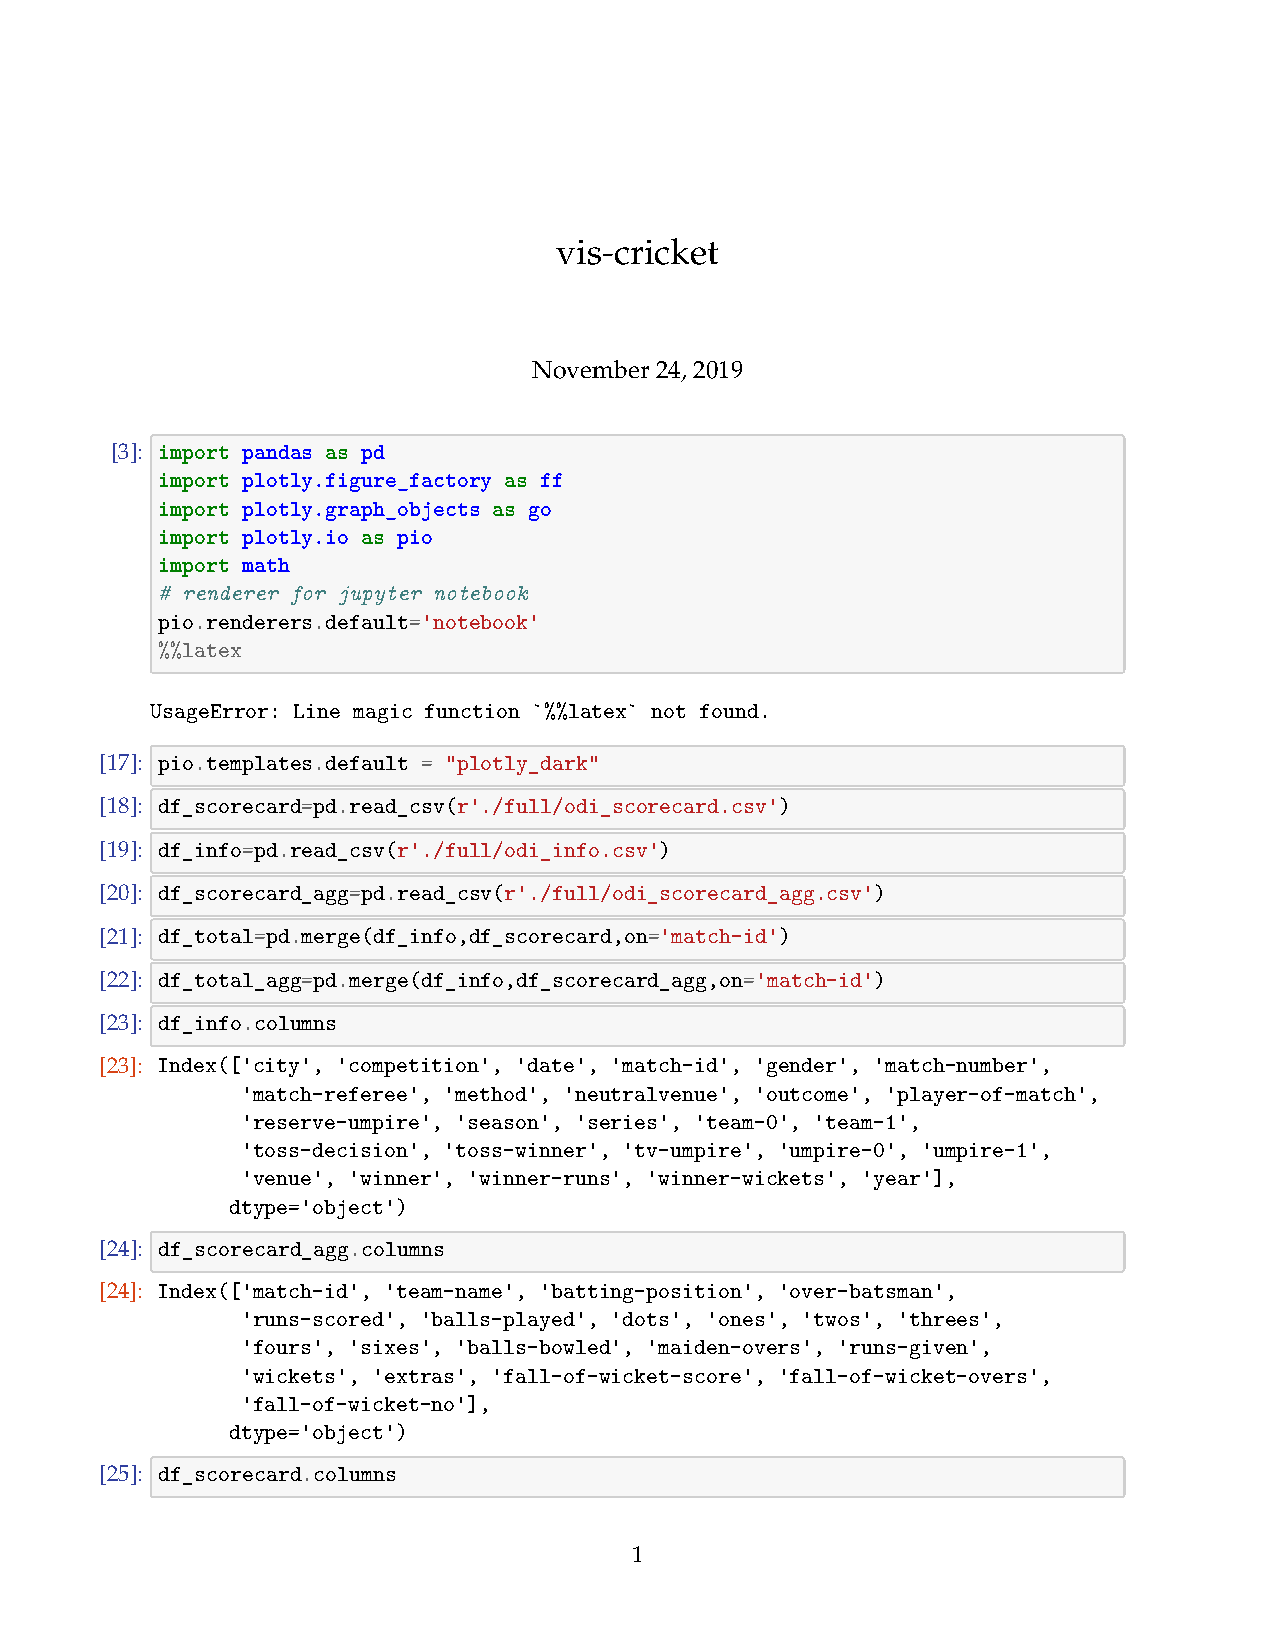
\includepdf[pages=-]{vis-cricket.pdf}
The interactive visualizations cannot be shown in LaTex therfore, here is the link for all the Jupyter notebook: \href{https://github.com/dev-SB/cricket-bi/blob/master/hypothesis.ipynb}{hypothesis.ipynb}.
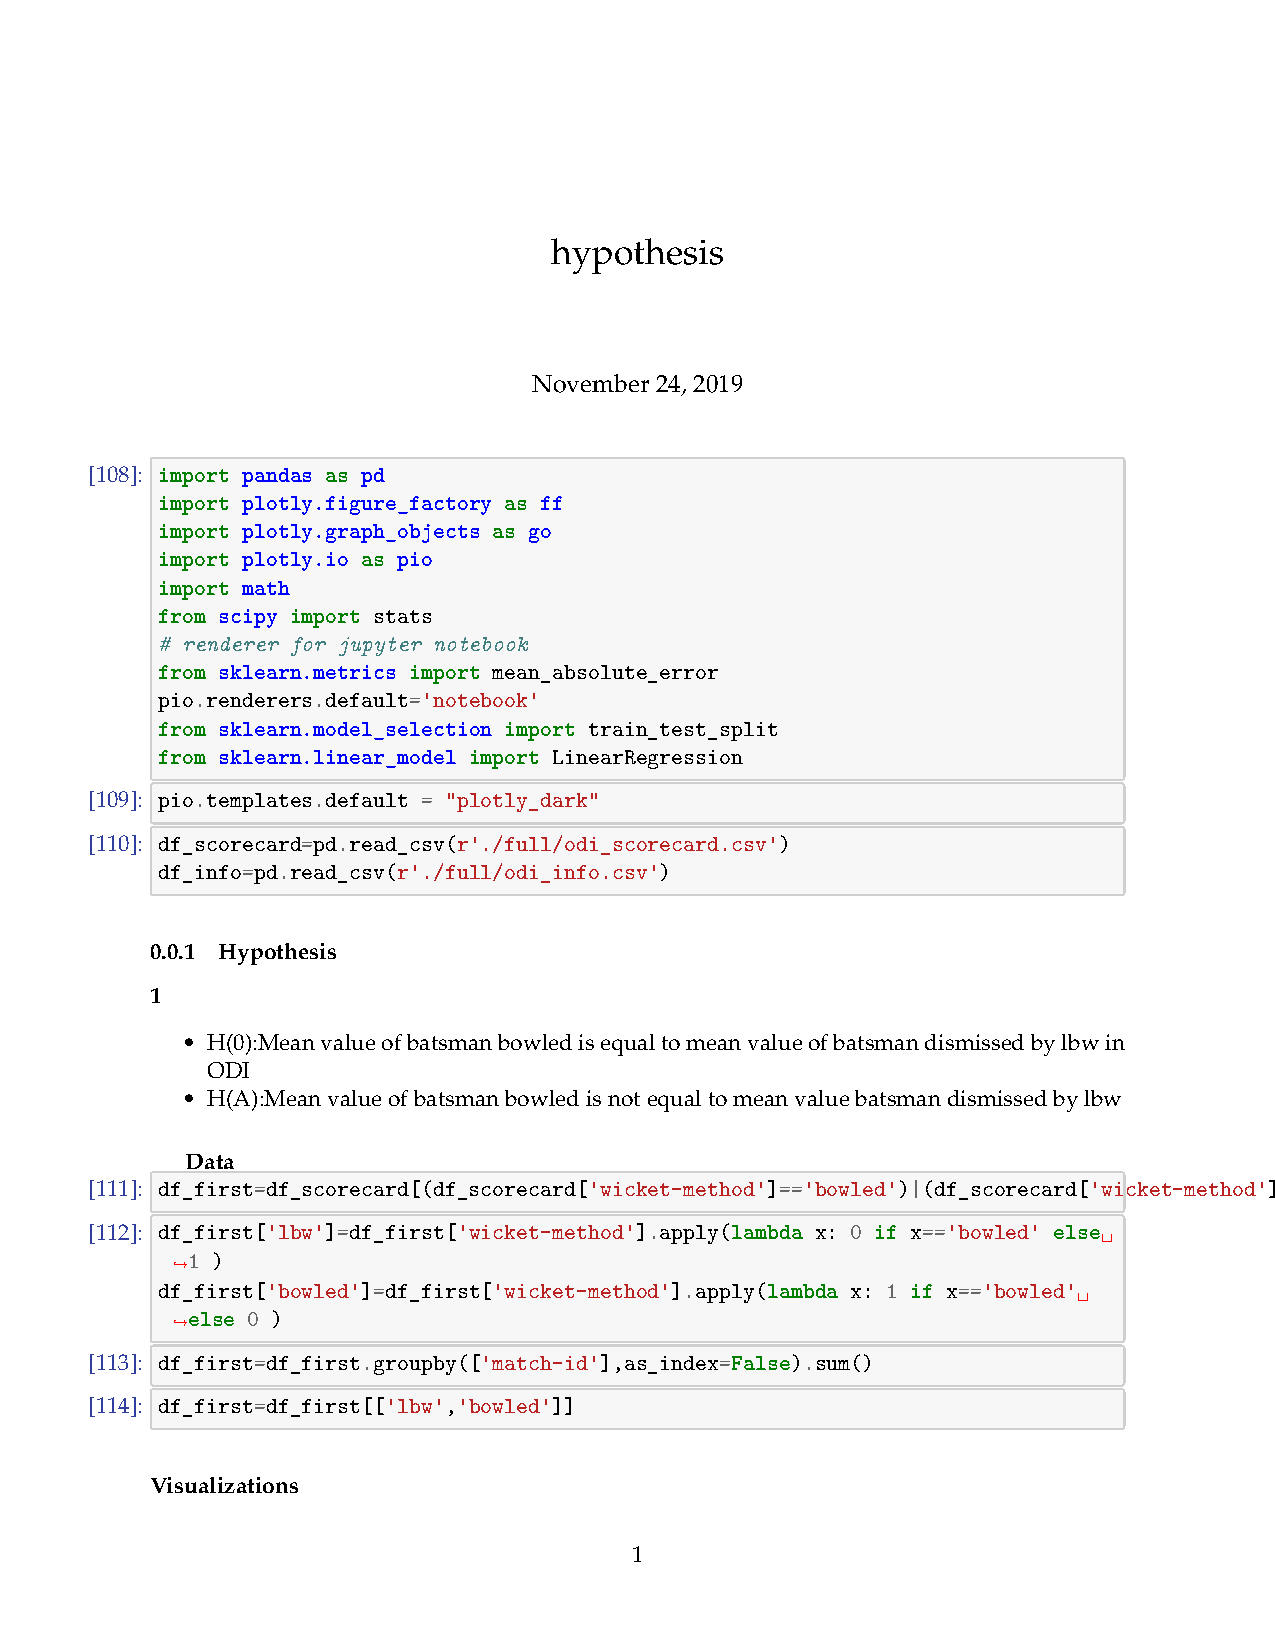
\includepdf[pages=-]{hypothesis-nb.pdf}
\end{document}